\documentclass[11pt,oneside,a4paper,titlepage,onecolumn]{article}

\usepackage[utf8]{inputenc}
\usepackage{textcomp}
\usepackage[official]{eurosym}
\usepackage[polish]{babel}
\usepackage{amsthm}
\usepackage{graphicx}
\usepackage[T1]{fontenc}
\usepackage{scrextend}
\usepackage{hyperref}
\usepackage{xcolor}
% \usepackage{nameref}
% \usepackage{showlabels}
% \usepackage{titlesec}
\usepackage{geometry}
\geometry{a4paper, portrait, margin=2cm}
\graphicspath{ {./fig/} }
\usepackage{listings}

\newenvironment{enumreq}
{ \begin{enumerate}[topsep=0pt,itemsep=-1ex,partopsep=1ex,parsep=1ex] }
{ \end{enumerate}                  } 


\setcounter{secnumdepth}{4}

%% Author and title
\author{Marek Marecki \and Krzysztof Franek}
\title{%
    Proving viability of Viua VM \\
    \large Implementation of high-level language on Viua VM\\
    and deployment of simple application \\
    ~\\
    Projekt Systemu\\
    dla języka Viuact}

\begin{document}

\lstset{basicstyle=\ttfamily,
columns=fixed}

\maketitle
{\footnotesize
\begin{center}
  \begin{tabular}{ | l | l | l | }
    \hline
    \parbox[t]{6.5cm}{\textbf{Temat pracy i akronim projektu:}\\Proving viablity of Viua VM (VVIA)} & \parbox[t]{4.5cm}{\textbf{Zleceniodawca:}\\\colorbox{yellow}{Nieznany}} & \parbox[t]{4.5cm}{\textbf{Konsultant:}\\\colorbox{yellow}{Nieznany}} \\ \hline
    \parbox[t]{6.5cm}{\textbf{Zespół projektowy:}\\Krzysztof Franek, Marek Marecki} & \parbox[t]{4.5cm}{\textbf{Kierownik projektu:}\\Marek Marecki} & \parbox[t]{4.5cm}{\textbf{Opiekun projektu:}\\dr hab. Marek A. Bednarczyk, prof. PJWSTK} \\ \hline
    \parbox[t]{3.5cm}{\textbf{Kierownik projektu:}\\Marek Marecki} &
      \multicolumn{2}{|l|}{\parbox[t]{9cm}{\textbf{Odpowiedzialny za dokument:}\\Marek Marecki}} \\ 
    \hline
  \end{tabular}
\end{center}
}

\tableofcontents
\newpage

\section{Architektura}

\subsection{Użyte wzorce projektowe -- Sposób konstrukcji kompilatora}

\begin{figure}[!htp]
    \centering
    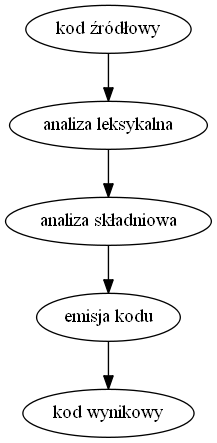
\includegraphics[width=5cm]{basic-compiler-flow}
    \caption{Podstawowy schemat budowy kompilatora}
    \label{basic_compiler_flow}
\end{figure}

Na rysunku \ref{basic_compiler_flow} przedstawiony jest uproszczony schemat budowy kompilatora.
W kompilatorach ''produkcyjnych'' (np. GCC, Clang, czy ICC) tych faz jest więcej -- przede wszystkim etap
emisji kodu jest dużo bardziej rozbudowany, oraz dochodzą etapy analizy semantycznej (czy program ma sens) czy
optymalizacji (prób takiego przekształcenia kodu programu żeby przy zachowaniu znaczenia działał wydajniej).

Kompilator języka ViuAct dostarczany jako element tej pracy inżynierskiej jest pozbawiony etapów
analizy semantycznej oraz optymalizacji. Analiza semantyczna (oraz weryfikacja typów i wykrywanie błędów na
etapie kompilacji) jest oddelegowana do assemblera dostarczanego przez platformę. Optymalizacja jest
całkowicie pominięta gdyż jest to temat niezwykle rozległy; implementacja i doszlifowanie algorytmów
optymalizujących kod jest sama w sobie materiałem wystarczającym na napisanie osobnej pracy inżynierskiej.

Architektura kompilatora języka ViuAct jest dokładniej opisana w rozdziale
\ref{architektura_kompilatora_viuact} (\nameref{architektura_kompilatora_viuact}) na
stronie \pageref{architektura_kompilatora_viuact}.
Sposób działania kompilatora jest opisany w rozdziale \ref{opis_etapow_kompilacji}
(\nameref{opis_etapow_kompilacji}) na stronie \pageref{opis_etapow_kompilacji}.
Omówienie interakcji kompilatora języka ViuAct z narzędziami dostarczanymi przez platformę Viua VM znajduje
się w rozdziale \ref{architektura_systemu} (\nameref{architektura_systemu}) na stronie
\pageref{architektura_systemu}.

Oprócz kompilatora (rozdział \ref{opis_kompilatora} na stronie \pageref{opis_kompilatora}) dostarczany jest
również ''program łączący'' (rozdział \ref{opis_linkera} na stronie \pageref{opis_linkera}) dokonujący
automatycznego połączenia wymaganych modułów w gotowy plik wykonywalny.

\newpage

\subsection{Architektura systemu}
\label{architektura_systemu}

Rysunek \ref{schemat_interakcji_viuact_z_viuavm} (''\nameref{schemat_interakcji_viuact_z_viuavm}'') prezentuje
schemat interakcji jakie zachodzą w całym systemie od momentu wczytania pliku źródłowego przez kompilator do
uruchomienia programu przez jądro Viua VM.

Ostatnią fazą jaką zajmuje się kompilator języka ViuAct dostarczany jako element tej pracy inżynierskiej jest
emisja kodu (''Assembly code emission''), której wynikiem jest plik z kodem źródłowym w języku assemblera Viua
VM (''\texttt{hello\_world.asm}'' na rysunku). Rozdział \ref{architektura_kompilatora_viuact}
(\nameref{architektura_kompilatora_viuact}) dokładniej opisuje działanie samego kompilatora.

\begin{figure}[!htp]
    \centering
    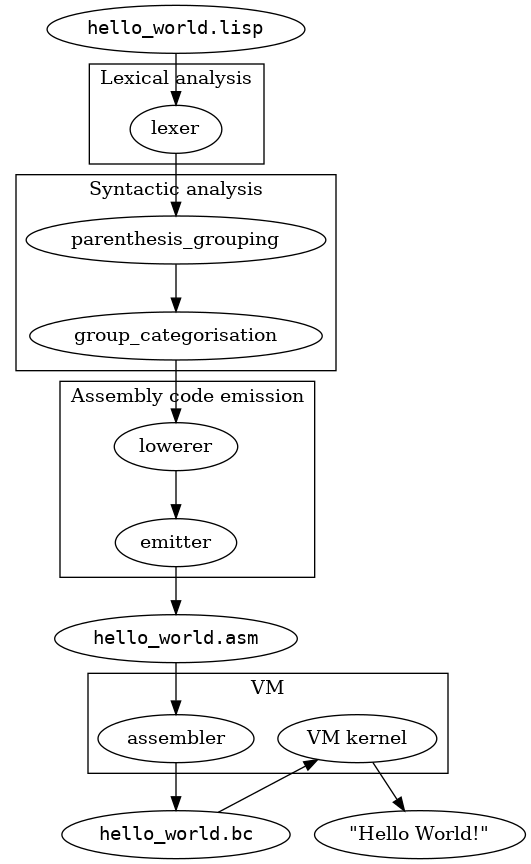
\includegraphics[width=9cm]{viuact-pipeline}
    \caption{Interakcje: od pliku źródłowego do działającego programu}
    \label{schemat_interakcji_viuact_z_viuavm}
\end{figure}

Zakres pracy inżynierskiej obejmuje wygenerowanie pliku zawierającego poprawny kod w języku
assemblera Viua VM oraz plików pomocniczych (zadanie kompilatora), oraz takim pokierowaniu
narzędziami dostarczanymi przez platformę, żeby wyemitowały one plik wykonywalny bądź bibliotekę (zadanie
''programu łączącego''). Zakładamy, że narzędzia dostarczane przez platformę działają poprawnie.

Pliki pomocnicze są wymagane przez ''program łączący'' (opisany w rozdziale \ref{opis_linkera} na stronie
\pageref{opis_linkera}). Ich dokładniejsze opisy znajdują się w rozdziałach
''\nameref{pliki_interfejsow_modulow}'' na stronie \pageref{pliki_interfejsow_modulow} i
''\nameref{pliki_zaleznosci_modulow}'' na stronie \pageref{pliki_zaleznosci_modulow}

\subsection{Dekompozycja systemu na podsystemy}
\label{architektura_kompilatora_viuact}

Język ViuAct jest implementowany przez dwa programy:

\begin{enumerate}
    \item \textbf{kompilator} - który przetwarza kod źródłowy w języku ViuAct na kod źródłowy w języku
        assemblera Viua VM
    \item \textbf{linker} - który na podstawie wyników pracy kompilatora tworzy pliki wykonywalne, które
        mogą być uruchomione na jądrze Viua VM
\end{enumerate}

Większość pracy w tym układzie wykonuje kompilator, opisany w rozdziale \ref{opis_kompilatora} na stronie
\pageref{opis_kompilatora}. Generuje on pliki zawierające kod źródłowy w języku assemblera gotowe do
przetworzenia przez assembler Viua VM na formę binarną, oraz pliki pomocnicze.

Z plików pomocniczych korzysta zarówno sam kompilator (do określenia interfejsów modułów importowanych przez
aktualnie kompilowany moduł), ale też linker -- do określenia jakie moduły powinny być dołączone do aktualnie
emitowanego pliku wykonywalnego, aby zapewnić dostępność wszystkich wymaganych funkcji. Linker jest dokładniej
opisany w rozdziale \ref{opis_linkera} na stronie \pageref{opis_linkera}.

\subsubsection{Kompilator -- \texttt{viuact-cc}}
\label{opis_kompilatora}

Kompilator składa się z kilku podsystemów, zgodnie z
przedstawieniem na rysunku \ref{ogolny_schemat_kompilatora_viuact}.

\begin{figure}[!htp]
    \centering
    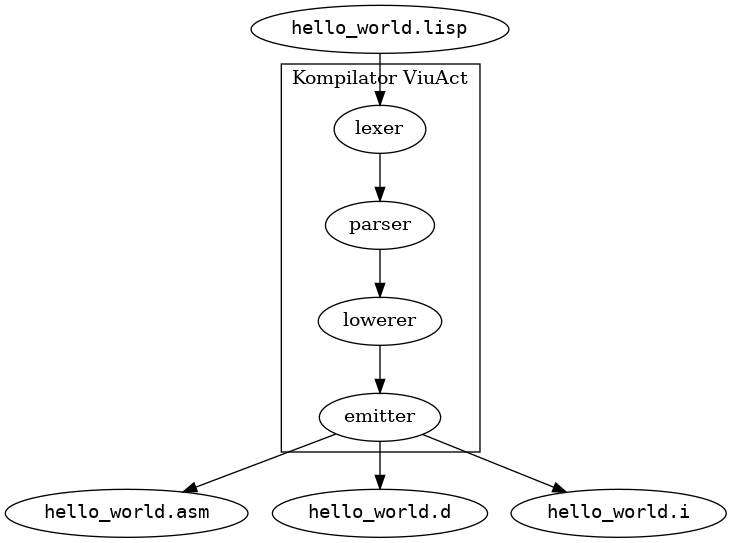
\includegraphics[width=10cm]{viuact-ogolny-schemat-kompilatora}
    \caption{Podział kompilatora na podsystemy}
    \label{ogolny_schemat_kompilatora_viuact}
\end{figure}

Każdy podsystem implementuje jedną z faz kompilacji:

\begin{enumerate}
    \item \textbf{lexer} dokonuje analizy leksykalnej wczytanego pliku źródłowego, dzieląc go na listę tokenów
    \item \textbf{parser} dokonuje analizy składniowej łącząc tokeny w grupy reprezentujące większe
        konstrukcje językowe
    \item \textbf{lowerer} mapuje grupy wyprodukowane przez \emph{parser} do odpowiednich funkcji
        \emph{emittera}; jest to dość banalny etap, ale upraszcza budowę kompilatora
    \item \textbf{emitter} tłumaczy konstrukcje językowe ViuAct na równoznaczne konstrukcje w języku
        assemblera Viua VM
\end{enumerate}

Różnica między podsystemami \emph{lowerer} i \emph{emitter} może być niejasna. Oba biorą udział w emisji
kodu wynikowego, ale \emph{lowerer} bezpośrednio zajmuje się tylko modułami i funkcjami, natomiast
\emph{emitter} implementuje emisję pojedynczych wyrażeń języka ViuAct -- przypisań \texttt{let}, konstrukcji
warunkowych \texttt{if}, wywołań funkcji, itd.

Proces kompilacji dokłaniej opisany jest w rozdziale \ref{opis_etapow_kompilacji}
(\nameref{opis_etapow_kompilacji}) na stronie \pageref{opis_etapow_kompilacji}.

\subsubsection{Program łączący -- \texttt{viuact-opt}}
\label{opis_linkera}

Program łączący (tzw. ''\emph{linker}'') zajmuje się finalną fazę ''kompilacji''.
Jest to stwierdzenie o tyle trafne, co niepoprawne. Zazwyczaj jednak nie ma to znaczenia, ponieważ zarówno
linker jak i kompilator jest ukrywany przed programistą. Popularne ''kompilatory'' jak np \emph{\texttt{g++}}
z GCC to tak naprawdę ''drivery''; wywołanie polecenia \emph{\texttt{g++}} powoduje wywołanie zarówno
kompilatora (\emph{\texttt{cc1}}), assemblera (\emph{\texttt{as}}), jak i linkera (\emph{\texttt{ld}}) w taki
sposób aby na wyjściu uzyskać oczekiwany wynik, czyli na przykład plik wykonywalny w formacie
ELF \emph{\texttt{a.out}}.

W przypadku kompilatora ViuAct proces ten wygląda podobnie, ale nie jest aż tak zautomatyzowany.
Rolę ''drivera'' pełni programista, który jest odpowiedzialny za wywołanie zarówno kompilatora jak i linkera.
Przykładowo:

\begin{lstlisting}
viuact-cc --mode exec ./hello_world.lisp
viuact-opt ./build/_default/hello_world.asm
\end{lstlisting}

Program łączący przeprowadzi proces asemblacji pliku podanego na wejściu, oraz dołączy do niego wszelkie
wymagane moduły. Zarówno asemblacja jak i łączenie będa przeprowadzone przez narzędzie dostarczane przez
platformę Viua VM -- \texttt{viuact-opt} zajmuje się jedynie wygenerowaniem odpowiednich poleceń dla tego
narzędzia.

Informacja o tym jakie moduły muszą zostać dołączone jest tworzona w oparciu o pliki zależności (opisane w
rozdziale \nameref{pliki_zaleznosci_modulow} na stronie \pageref{pliki_zaleznosci_modulow}).
Dla uproszczenia projektu program łączący nie zbiera informacji o zależnościach rekurencyjnie.

Po zebraniu informacji o zależnościach program łączący dokonuje asemblacji wszystkich modułów, od których
zależy kompilowany moduł główny. Następnie asembluje moduł główny i łączy wszystkie wyemitowane modułu
bytecode'u w gotowy plik wykonywalny.

\subsection{Przepieg procesu kompilacji}
\label{opis_etapow_kompilacji}

Co po kolei robi kompilator.
Od wczytania pliku z kodem źródłowym do wyemitowania kodu wynikowego w języku assemblera.

\section{Projekt struktury}

\subsection{Diagram klas}

Brak diagramu klas, ponieważ program nie jest pisany w stylu obiektowym.

\section{Decyzje projektowe}

\subsection{Środowisko docelowe}

\subsection{Środowisko implementacji}

\subsection{Priorytety implementacyjne}

Maksymalizacja prostoty budowy kompilatora i języka.
Marginalizacja obsługi błędów w kompilatorze z uwagi na brak czasu.
Marginalizacja optymalizacji z uwagi na brak czasu.

\section{Projekt algorytmów i przyjętych protokołów}

\section{Projekt rozwiązań sprzętowych}

Brak w tym projekcie. Jest on wyłącznie softwareowy.

\section{Projekt interfejsu}

\subsection{Interfejs użytkownika}

\subsubsection{Założenia konstrukcji interfejsu}

\subsection{Interfejs kompilatora}

Kompilator składa się z dwóch programów: \texttt{viuact-cc} (kompilatora właściwego) i \texttt{viuact-opt}
(programu łączącego).

\subsection{Interfejs języka}

Interfejsem języka jest jego składnia.
Jest ona opisana w specyfikacji języka.

\subsection{Inne interfejsy}

\subsubsection{Pliki interfejsów modułów (\texttt{.i})}
\label{pliki_interfejsow_modulow}

\subsubsection{Pliki zależności modułów (\texttt{.d})}
\label{pliki_zaleznosci_modulow}

\section{Projekt bazy danych}

Brak bazy danych w projekcie.

\section{Opis implementacji}

Krótka dyskusja jak przyjęte rozwiązania projektowe spełniają wymagania, szczególnie jakościowe, np.
bezpieczeństwo.

\section{Słownik pojęć}

\begin{description}
    \item[kompilator] program tłumaczący kod w jednym języku (zazwyczaj wysokiego poziomu) na kod o takim
        samym znaczeniu w innym języku (zazwyczaj niższego poziomu)
    \item[jednostka translacji] w przypadku języka ViuAct jest to pojedynczy moduł
    \item[linker] program łączący wiele modułów w plik wykonywalny
    \item[plik wykonywalny] plik zawierający bytecode w formacie, który może zostać wykonany przez jądro Viua
        VM
    \item[moduł] w załeżności od kontekstu: \emph{1/} kod źródłowy modułu w języku ViuAct, lub \emph{2/} plik
        zawierający bytecode w formacie, który może zostać wykorzystany przez linker bądź jądro Viua VM do
        dołączenia
    \item[biblioteka] zbiór modułów bytecode'u
    \item[jądro] podsystem Viua VM odpowiadający za uruchamianie programów (tzw. ''\emph{kernel}'')
\end{description}

\section{Załączniki}

Specyfikacja języka ViuAct -- ''\emph{viuact-specification.pdf}''.

\end{document}
